\documentclass[9pt, aspectratio=169]{beamer}

\usetheme{metropolis}
\setbeamertemplate{itemize items}{\faAngleRight}

\metroset{titleformat=smallcaps,block=fill,numbering=counter,progressbar=frametitle,sectionpage=none}
\setbeamersize{text margin left=5mm,text margin right=5mm} 
% \input{embed_video}
\usepackage{fontspec,minted}
\usepackage[scale=1]{ccicons}
\usepackage{metalogo}
\usepackage{xcolor,colortbl}
\usepackage{multicol,multirow,booktabs}
\usepackage{appendixnumberbeamer}
\usepackage{graphicx}
\usepackage{mismath}
\usepackage{bm}
\usepackage{fontawesome5}
\usepackage{csquotes}
\usepackage[backend=biber, natbib, sorting=nyt, doi=true, url=false, url=false, isbn=false, maxbibnames=10]{biblatex}
\addbibresource{../utils/refs.bib}

\usepackage[spanish, es-nodecimaldot]{babel}
\deftranslation[to=spanish]{Definition}{Definición}
\deftranslation[to=spanish]{Theorem}{Teorema}
\deftranslation[to=spanish]{Example}{Ejemplo}

\usepackage{mathtools, mathrsfs}
\usefonttheme{professionalfonts}
\usepackage{textcomp, wasysym}

\setsansfont[BoldFont={Iwona Heavy}, Numbers={Lining, Proportional}]{Iwona Light}
\setmonofont[Scale=MatchLowercase]{Hack Nerd Font Mono}

\setbeamercolor{alerted text}{fg=red,bg=black!2}
\setbeamercolor{progress bar}{fg=red,bg=red!2}
\setbeamertemplate{itemize item}{\faCaretRight}
\setbeamertemplate{itemize subitem}{ \faAngleRight}
\setbeamertemplate{blocks}[shadow=false]
\setbeamercolor{block title}{bg=black!30,fg=red}
\setbeamercolor{block body}{bg=black!20,fg=black}
\setbeamertemplate{theorem begin}
{%
\begin{\inserttheoremblockenv}
{%
\inserttheoremheadfont
%{Teorema:}
\inserttheoremname
\ifx\inserttheoremaddition\@empty\else\ : \inserttheoremaddition\fi%
\inserttheorempunctuation
}%
}
\setbeamertemplate{theorem end}{\end{\inserttheoremblockenv}}
\makeatother


 
\usepackage{gensymb,amssymb}
\usepackage{siunitx}
\DeclareSIUnit{\nada}{\relax}
\usepackage{upquote}
\usepackage{cancel}
\usepackage{algpseudocode}
\algrenewcommand\algorithmicrequire{\textbf{Requiere}}
\algrenewcommand\algorithmicensure{\textbf{Devuelve}}
\setbeamertemplate{blocks}[shadow=false]

\newcommand{\cx}{\column{0.5\textwidth}}
\newcommand{\cw}[1]{\column{#1\textwidth}}

\author{Manuel Carlevaro}
\date{{\tiny Departamento de Ingeniería Mecánica \\
             Grupo de Materiales Granulares - UTN FRLP \\
             manuel.carlevaro@gmail.com }}
\institute{
  \vspace{6em}
  \centering
  {\tiny
  Cálculo Avanzado \enspace • \enspace 2025 \\
    \faLinux \- $\cdot$ \- \fontspec{TeX Gyre Pagella}\XeLaTeX \- $\cdot$ \- \ccbysa }
}

%% Operadores
\DeclareMathOperator{\sen}{sen}
\DeclareMathOperator{\senc}{senc}
\DeclareMathOperator{\sign}{sign}
\DeclareMathOperator{\Tr}{Tr}
\DeclareMathOperator{\rg}{rg}
\DeclareMathOperator{\cond}{cond}
\newcommand{\T}[1]{\underline{\bm{#1}}}
\newcommand{\uvec}[1]{\hat{\bm{#1}}}

\usepackage{hyperref}
\hypersetup{
    colorlinks,
    citecolor=blue,
    filecolor=black,
    linkcolor=blue,
    urlcolor=blue
}
\urlstyle{same}

%% Códigos
\usepackage{minted}
\newminted[cpp]{cpp}{linenos,fontsize=\footnotesize,frame=lines,numbersep=4pt}
\newmintedfile[cppcode]{cpp}{linenos,fontsize=\footnotesize,frame=lines,numbersep=4pt}
\newcommand{\mic}[1]{\mintinline{C++}{#1}}

\newminted[py]{python}{linenos,fontsize=\footnotesize,frame=lines,numbersep=4pt}
\newminted[pyc]{pycon}{linenos,fontsize=\footnotesize,frame=lines,numbersep=4pt} % Consola de Python
\newminted[ipy3]{ipython3}{linenos,fontsize=\footnotesize,frame=lines,numbersep=4pt} % Consola de iPython3
\newmintedfile[pycode]{python}{linenos,fontsize=\footnotesize,frame=lines,numbersep=4pt}

\newmintedfile[makef]{basemake}{linenos,fontsize=\footnotesize,frame=lines,numbersep=4pt}
\definecolor{bg}{RGB}{22,43,58}
\newminted[shell]{console}{linenos=false,fontsize=\footnotesize,breaklines=true, frame=single} % Linea de comandos
\renewcommand\listingscaption{Código}

\makeatletter
\AtBeginEnvironment{minted}{\dontdofcolorbox}
\def\dontdofcolorbox{\renewcommand\fcolorbox[4][]{##4}}
\makeatother

% uso:
% Ejemplo de uso explícito:
% \begin{py}
% >>> list("abcd")
% ['a', 'b', 'c', 'd']
% \end{py}
% 
% Ahora ejemplo de código en file:
% \pycode{Chapters/intro/code/hola.py}
% 
% También se puede poner un sector del file:
% \pycode[firstline=6, lastline=7]{Chapters/intro/code/hola.py}
% 
% También se puede poner código \textit{inline}: \mip{print('¡Hola mundo!')} y en una sola línea:
% \slp|if __name__ == '__main__')|
% 
% Por último, se puede poner el código en un entorno \textit{float}, esto es, como las tablas y las figuras, con un caption y un label para luego hacer referencias, como por ejemplo al Código \ref{code:hola}.


\usepackage{tikz}
\usetikzlibrary{shapes,shadows,arrows,positioning,matrix,chains,backgrounds,fit}

\tikzset{
    %Define standard arrow tip
    >=stealth',
    %Define style for boxes
    obj/.style={
           rectangle,
           rounded corners,
           draw, very thick,
           text width=10em, fill=green!20,
           minimum height=2em,
           text centered, drop shadow},
    proc/.style={
	    rectangle, rounded corners,
	    draw,fill=red!50,very thick,
	    text width=8em,minimum height=2em,
	    text centered, drop shadow},
    % Define arrow style
    pil/.style={
           ->,
           thick,
           shorten <=2pt,
           shorten >=2pt,}
}

\setbeamertemplate{bibliography item}{%
  \ifboolexpr{ test {\ifentrytype{book}} or test {\ifentrytype{mvbook}}
    or test {\ifentrytype{collection}} or test {\ifentrytype{mvcollection}}
    or test {\ifentrytype{reference}} or test {\ifentrytype{mvreference}} }
    {\setbeamertemplate{bibliography item}{\faBook}}
    {\ifentrytype{online}
            {\setbeamertemplate{bibliography item}{\faGlobe}}
   {\setbeamertemplate{bibliography item}{\faFileText}}}%
  \usebeamertemplate{bibliography item}}

\defbibenvironment{bibliography}
  {\list{}
     {\settowidth{\labelwidth}{\usebeamertemplate{bibliography item}}%
      \setlength{\leftmargin}{\labelwidth}%
      \setlength{\labelsep}{\biblabelsep}%
      \addtolength{\leftmargin}{\labelsep}%
      \setlength{\itemsep}{\bibitemsep}%
      \setlength{\parsep}{\bibparsep}}}
  {\endlist}
  {\item}
\newcommand{\bcite}[1]{\citeauthor{#1}, \citetitle{#1} (\citeyear{#1})}


\title{Introducción a la variable compleja}
\subtitle{¡Bienvenid@s! Números complejos (repaso). Funciones de variable compleja. Límite y continuidad. Diferenciabilidad y funciones analíticas. Integración en el campo complejo. Sucesiones y series.}
% \subtitle{Introducción al curso.\\ Números complejos (repaso). Funciones de variable compleja. Límite y continuidad. Diferenciabilidad y funciones analíticas.}

% ver: 
% https://www.youtube.com/watch?v=BOx8LRyr8mU
% https://www.youtube.com/watch?v=rVvGqWyQB_0
% Herbert Gross
% Calculus cof Complex Variables, ...
%


\begin{document}
\maketitle

\begin{frame}{ ¡Bienvenid@s! }
	\begin{columns}[c]
		\cx
		\textbf{Docentes:}
		\begin{itemize}
			\item Profesor: Manuel Carlevaro
			\item Ayudante de Primera: Christian Molina
		\end{itemize}
		\vspace{1em}

		\textbf{Clases:}
		\begin{itemize}
			\item Miércoles de 17:00 a 19:15
			\item Teoría + práctica
			\item Clases de consulta:
			      \begin{itemize}
				      \item MC: Miércoles 15 a 16 hs.
				      \item CM: A coordinar.
			      \end{itemize}
		\end{itemize}
		\cx
		\textbf{Evaluación:}
		\begin{itemize}
			\item Parciales 2 (+ 2 recuperatorios) + Instancia evaluativa complementaria (febrero 2026)
			\item Aprobación directa: 2 parciales ($\geq 6$)
			\item Aprobación no directa - examen final: al menos un parcial con 4 o 5
		\end{itemize}
	\end{columns}
\end{frame}

\begin{frame}{Programa}
	\begin{columns}[t]
		\cx
		\begin{enumerate}
			\item Introducción a la variable compleja (2 clases)
			\item Transformada y serie de Fourier (2 clases)
			\item Transformada de Laplace (1 clase)
			\item Errores en el cálculo numérico (1 clase)
			\item Cálculo de raíces: soluciones de una variable (2 clases)
			\item Normas de vectores y matrices (2 clases)
		\end{enumerate}
		\cx
		\begin{enumerate}
			\setcounter{enumi}{6}
			\item Autovalores y autovectores (2 clases)
			\item Resolución de sistemas de ecuaciones lineales (2 clases)
			\item Aproximación discreta y continua por el método de los mínimos cuadrados (dos clases)
			\item Resolución de problemas de valor inicial (dos clases)
			\item Resolución de problemas de contorno (dos clases)
			\item Resolución de ecuaciones diferenciales de segundo orden mediante diferencias finitas (2 clases)
		\end{enumerate}
	\end{columns}
	\vspace{1em}
	\begin{columns}[c]
		\cx
		\centering
		\only<1>{\phantom{\alert{Primer parcial: 12/07} }}
		\only<2>{\alert{Primer parcial: 25/6,\\ recuperatorios: 16/7 y 6/8.} }

		\cx
		\centering
		\only<1>{\phantom{\alert{Segundo parcial: 22/11} }}
		\only<2>{\alert{Segundo parcial: 03/12, \\ recuperatorios: 10/12 y 17/12 (?).} }
	\end{columns}
\end{frame}

\begin{frame}{Recursos}
	\textbf{Específicos de Cálculo Avanzado:}
	\begin{itemize}
		\item CVG: \href{https://frlp.cvg.utn.edu.ar/course/view.php?id=189}{Cálculo Avanzado}
		\item GitHub: \url{https://github.com/manuxch/calculo_avanzado}
	\end{itemize}

	\textbf{Recursos adicionales:}
	\begin{itemize}
		\item Python y programación: \url{https://github.com/gmg-utn/compTools}
		\item \LaTeX - \XeLaTeX: \url{https://es.wikibooks.org/wiki/Manual_de_LaTeX}
	\end{itemize}
\end{frame}

\begin{frame}{Bibliografía}
	\begin{columns}[t]
		\cw{0.45}
		\begin{itemize}
			{ \small
			\item \fullcite{kreyszig2011}.
			\item \fullcite{spiegel2011}.
			\item \fullcite{brown2004}.
			\item \fullcite{oneil2012}.
			\item \fullcite{edwards2009}.
			      }
		\end{itemize}

		\cw{0.45}
		\begin{itemize}
			{ \small
			\item \fullcite{burden2017}.
			\item \fullcite{gupta2019}.
			\item \fullcite{strang2006}.
			\item \fullcite{pine2019}.
			\item \fullcite{batista2023}.
			      }
		\end{itemize}
	\end{columns}
\end{frame}

\begin{frame}[standout]
	\centering
	¿Preguntas, dudas, comentarios?
\end{frame}

\section{Número complejos}

\begin{frame}{Los números complejos}
	\begin{columns}[t]
		\cw{0.3}
		Sistema de enteros:
		\begin{align*}
			2 x & = 3   \\
			x   & = \;?
		\end{align*}

		Números ``reales'': $\{ x: x^2 \geq 0\}$
		\begin{align*}
			x^2 & = -1  \\
			x   & = \;?
		\end{align*}

		Motivación: $ x^2 + 1 = 0 $ ¿tiene solución?

		Ejemplo: usar $y = e^{rx}$ para resolver:
		\[  y'' + y = 0 \]
		\pause

		\cw{0.3}
		\begin{align*}
			 & r^2 e^{rx} + e^{rx} = 0                                     \\
			 & \therefore r^2 + 1 = 0 \therefore r = \pm \sqrt{-1} = \pm i \\
			 & \therefore y = e^{ix} \text{ o } y = e^{-ix}                \\
			 & \boxed{y = \cos x \text{ o } y = \sen x}
		\end{align*}

		De ``alguna manera'' $i$ debe existir y $e^{ix}$ debe estar relacionado a $\sen x$ y $\cos x$.
		\pause
		\bigskip

		El sistema de \alert{números complejos}:
		\[ \mathbb{C} = \{ x + i y : x \text{ y } y \text{ son reales.} \} \]
		con la estructura:
		\begin{align*}
			(1)   & \; x_1 + i y_1 = x_2 + i y_2 \Leftrightarrow \\
			\quad & x_1 = x_2 \text{ y } y_1 = y_2               \\
		\end{align*}

		\cw{0.3}
		\begin{align*}
			(2)   & \; (x_1 + i y_1) + (x_2 + i y_2) = \\
			\quad & = (x_1 + x_2) + i (y_1 + y_2)      \\
			(3)   & \; r(x + i y) = r x + i r y        \\
			\quad & r \text{ real.}                    \\
		\end{align*}

		\vspace{-2em}
		$\therefore$ los números complejos son un \alert{espacio vectorial} por definición.
		\bigskip

		\begin{center}
			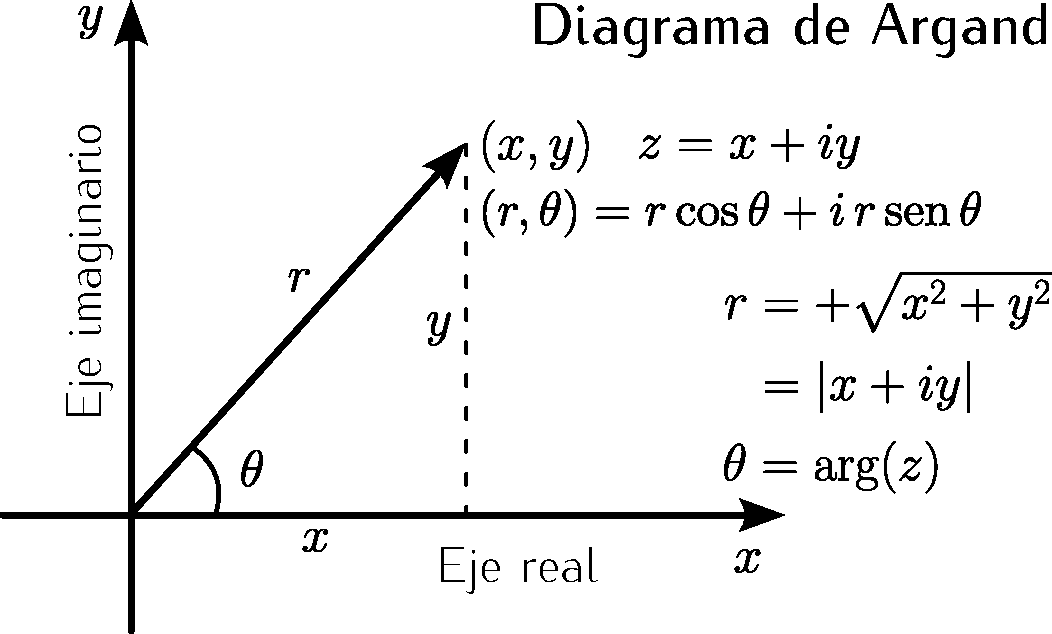
\includegraphics[width=1.0\textwidth]{figs/argand.pdf}
		\end{center}
	\end{columns}
\end{frame}

\begin{frame}
	\begin{columns}[t]
		\cw{0.25}
		Estructura adicional de $\mathbb{C}$:
		\begin{align*}
			(4) & \; (a + ib)(c + id) =     \\
			    & = (ac - bd) + i (bc + ad)
		\end{align*}
		Caso especial:
		\begin{align*}
			(a + ib)(a - ib) & = a^2 + b^2 \geq 0 \\
			                 & = |a + i b|^2
		\end{align*}
		\textbf{Definición:} el complejo conjugado de $z = x + y i$ es
		\[ \bar{z} = x - y i \]
		\begin{center}
			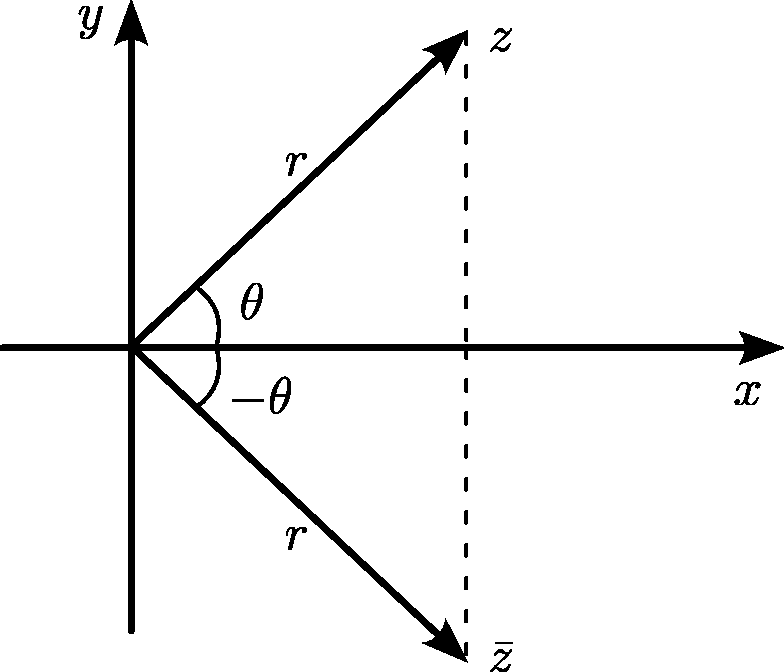
\includegraphics[scale=0.25]{figs/conjugado.pdf}
		\end{center}

		\cw{0.25}
		\begin{align*}
			\frac{c + di}{a + bi} & = \left(\frac{c + di}{a + bi}\right) \left(\frac{a - bi}{a - bi}\right) \\
			                      & = \frac{(ac + bd) + (ad - bc)i}{a^2 + b^2}
		\end{align*}
		\begin{align*}
			\frac{3 + 2 i}{4 + i} & = \frac{(3 + 2i)(4 - i)}{(4 + i)(4 - i)} \\
			                      & = \frac{14 + 5 i}{17}                    \\
			                      & = \frac{14}{17} + \frac{5}{17}i
		\end{align*}

		\[ \therefore \frac{\text{complejo}}{\text{complejo}} = \text{complejo} \]
		(excepto para división por cero).

		\cw{0.4}
		Producto en coordenadas polares:
		\begin{multline*}
			(r_1, \theta_1)(r_2, \theta_2) = (r_1 \cos \theta_1 + i r_1 \sen \theta_1) \\
			(r_2 \cos \theta_2 + i r_2 \sen \theta_2)= \\
			r_1 r_2 (\cos \theta_1 \cos \theta_2 - \sen \theta_1 \sen \theta_2) + \\
			i r_1 r_2 (\sen \theta_1 \cos \theta_2 + \sen \theta_2 \cos \theta_1) = \\
			r_1 r_2 \cos(\theta_1 + \theta_2) + i r_1 r_2 \sen(\theta_1 + \theta_2) = \\
			\boxed{ (r_1 r_2, \theta_1 + \theta_2) } \qquad
		\end{multline*}
		Por inducción:
		\begin{multline*}
			(r_1, \theta_1) \cdots (r_n, \theta_n) = \\
			(r_1 \cdots r_n, \theta_1 + \cdots + \theta_n)
		\end{multline*}
		Caso especial:
		\[ (r, \theta)^n = (r^n, n \theta) \]
		\[ \therefore r = 1 \rightarrow (1, \theta)^n = (1, n \theta) \]
	\end{columns}
\end{frame}


\begin{frame}
	\begin{columns}[t]
		\cx
		Teorema de De Moivre:
		\[  (\cos \theta + i \sen \theta)^n = \cos n \theta + i \sen n \theta \]

		Ejemplo:
		\begin{multline*}
			(\cos \theta + i \sen \theta)^2 = \cos 2 \theta + i \sen 2 \theta \\
			= (\cos^2 \theta - \sen^2 \theta) + i 2 \sen \theta \cos \theta \\
		\end{multline*}

		\begin{align*}
			\therefore \;\sen 2 \theta & = 2 \sen \theta \cos \theta     \\
			\cos 2 \theta              & = \cos^2 \theta - \sen^2 \theta
		\end{align*}


		\cx
		Raíces: encontrar $\sqrt{i}$
		\begin{equation*}
			\sqrt[6]{i} = x + i y \rightarrow i = (x + i y)^6 = 0 + 1 i
		\end{equation*}

		\begin{align*}
			\therefore \; & x^6 + 15 x^4 (iy)^2 + 15 x^2 (iy)^4 + (iy)^6  \onslide<2->{\textcolor{red}{ = 0}} \\
			              & + 6 x^5 (iy) + 20 x^3 (iy)^3 + 6x (iy)^5 \onslide<2->{\textcolor{red}{ = 1}}
		\end{align*}
		Sistema complicado a resolver:
		\begin{equation*}
			\begin{cases}
				x^6 + 15 x^4 (iy)^2 + 15 x^2 (iy)^4 + (iy)^6 = 0 \\
				6 x^5 (iy) + 20 x^3 (iy)^3 + 6x (iy)^5 = 1
			\end{cases}
		\end{equation*}
	\end{columns}
\end{frame}

\begin{frame}
	\begin{columns}[t]
		\cx
		En coordenadas polares:
		\begin{align*}
			 & i = (1, \pi/2) \therefore \; \sqrt[6]{i} = (r, \theta)                                              \\
			 & \rightarrow  i = (r, \theta)^6 = (r^6, 6 \theta)                                                    \\
			 & \therefore r = 1, \quad 6 \theta = \frac{\pi}{2} \textcolor{red}{+ 2 \pi k} = \frac{1 + 4 k}{2} \pi
		\end{align*}

		\begin{align*}
			r =      & 1,                                                                                                            \\
			\theta = & \frac{\pi}{12}, \frac{5 \pi}{12}, \frac{ 9 \pi}{12}, \frac{13 \pi}{12}, \frac{17 \pi}{12}, \frac{21 \pi}{12}, \\
			         & \frac{25 \pi}{12}, \cdots
		\end{align*}

		\begin{align*}
			\left( 1, \dfrac{3 \pi}{4} \right) & = \cos \dfrac{3 \pi}{4} + i \sen \dfrac{3 \pi}{4} \\
			                                   & = \frac{1}{\sqrt{2}} (-1 + i)
		\end{align*}


		\cx
		\begin{center}
			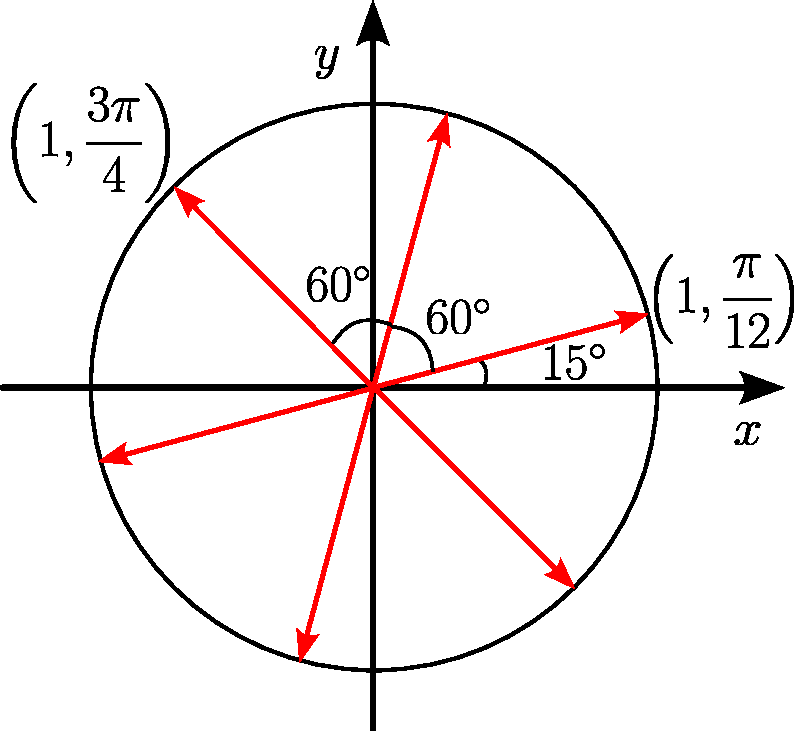
\includegraphics[scale=0.35]{figs/raices.pdf}
		\end{center}

		\begin{block}{Sistema de números complejos:}
			Los números complejos son \textbf{cerrados}
			respecto de la radicación.
		\end{block}
	\end{columns}
\end{frame}

\begin{frame}[standout]
	Pausa para resolver problemas: 1 -- 8.
\end{frame}


%%%%%%%%%%%%%%%%%%%%%%%%%%%%%%%%%%%%%%%%%%%%%%%%%%%%%%%%%%%%%%%%%%%%%%%%%
% Fuente de esta presentación:
%       https://youtu.be/rVvGqWyQB_0
% del curso:
%  Calculus Revisited: Complex Variables, Differential Equations, and Linear Algebra
%   https://ocw.mit.edu/courses/res-18-008-calculus-revisited-complex-variables-differential-equations-and-linear-algebra-fall-2011/
%%%%%%%%%%%%%%%%%%%%%%%%%%%%%%%%%%%%%%%%%%%%%%%%%%%%%%%%%%%%%%%%%%%%%%%%%


\section{Funciones de variable compleja}

\begin{frame}{Funciones de variable compleja}
	\begin{columns}[c]
		\cw{0.4}
		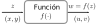
\includegraphics[width=0.9\textwidth]{figs/fig-01} \pause
		\cw{0.6}
		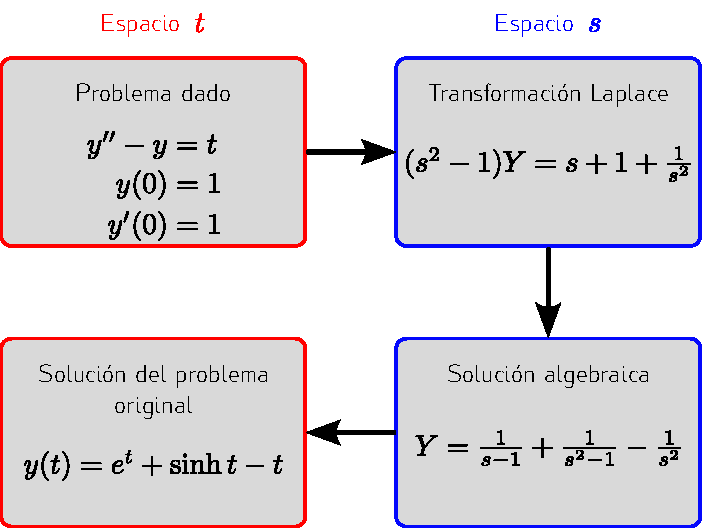
\includegraphics[width=0.9\textwidth]{figs/fig-02}
	\end{columns} \pause

	\begin{columns}[c]
		\cw{0.6}
		\begin{exampleblock}{Ejemplo:}
			\begin{align*}
				f(z)               & = z^2 = (x + iy)^2                             \\
				                   & = x^2 + 2 x i y + i^2 y^2 = x^2 - y^2 + 2 i xy \\
				\therefore f(x, y) & = (x^2 - y^2, 2xy)
			\end{align*}
		\end{exampleblock} \pause
		\cw{0.3}
		$\therefore f(z) = z^2$ es equivalente al \alert{sistema real}:
		\vspace{1em}
		\[
			\begin{cases*}
				u = x^2 + y^2 \\
				v = 2xy
			\end{cases*}
		\]
	\end{columns}
\end{frame}

\section{Límites}

\begin{frame}{Límites}
	$\mathbb{C}$: números complejos \\
	$f: \mathbb{C} \mapsto \mathbb{C}, a \in \mathbb{C}$

	\begin{columns}[c]
		\cw{0.5}
		\begin{alertblock}{Definición:}
			\[ \lim_{z \rightarrow a} f(z) = L \]

			dado $\epsilon >0$ existe $\delta > 0$ tal que
			\[ 0 < |z - a| < \delta \rightarrowtail |f(z) - L| < \epsilon \]
		\end{alertblock} \pause
		\cw{0.5}
		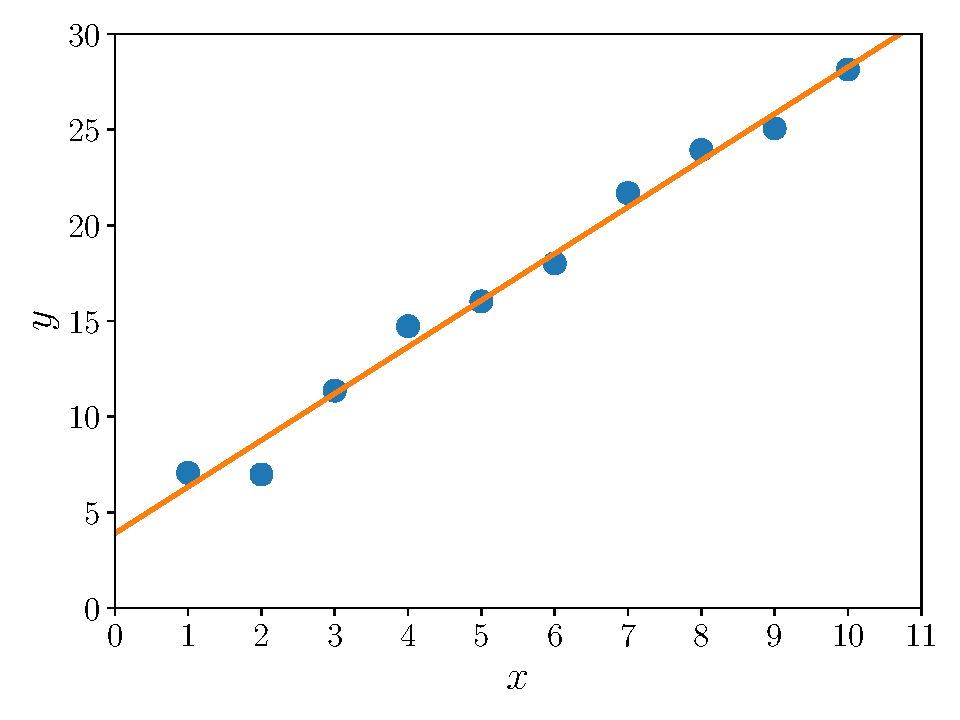
\includegraphics[width=0.9\textwidth]{figs/fig-03}
	\end{columns} \pause

	\noindent Los teoremas usuales sobre límites \alert{son válidos}. En particular: \vspace{0.5em}

	\begin{columns}[t]
		\cw{0.3}
		Si
		\begin{align*}
			f(z) & = u(x, y) + i v(x, y) \\
			L    & = L_1 + i L_2         \\
			a    & = a_1 + i a_2
		\end{align*}
		\cw{0.6}
		Entonces:
		\[ \lim_{z \rightarrow a} f(z) = L \longleftrightarrow
			\begin{cases}
				\lim_{(x,y) \rightarrow (a_1, a_2)} u(x, y) = L_1 \\
				\lim_{(x,y) \rightarrow (a_1, a_2)} v(x, y) = L_2
			\end{cases}
		\]
	\end{columns}
\end{frame}

\section{Derivadas de funciones complejas}

\begin{frame}{Derivada}
	\begin{columns}
		\cw{0.5}
		\begin{alertblock}{Definición:}
			\[ f'(z_0) = \lim_{\Delta z \rightarrow 0} \left[ \frac{f(z_0 + \Delta z) - f(z_0)}{\Delta z} \right] ¨ \]
		\end{alertblock} \pause
		\vspace{2em}

		Si $w = f(z) = u(x, y) + i v(x, y)$:
		\begin{align*}
			f'(z_0) & = \frac{dw}{dz} = \lim_{\Delta z \rightarrow 0} \frac{\Delta w}{\Delta z}                          \\
			        & = \lim_{\Delta z \rightarrow 0} \left[ \frac{\Delta u + i \Delta v}{\Delta x + i \Delta y} \right]
		\end{align*} \pause

		\cw{0.5}
		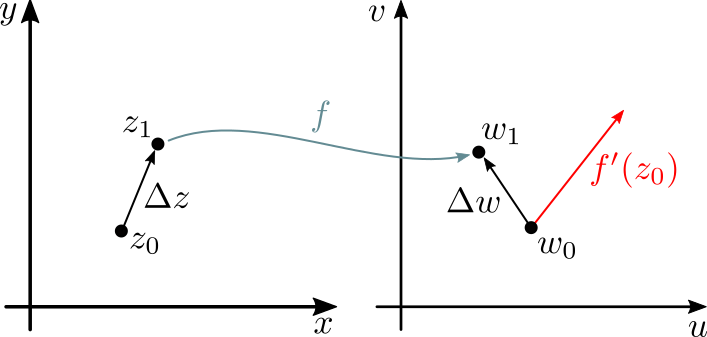
\includegraphics[width=0.9\textwidth]{figs/fig-04b.png}
	\end{columns}
\end{frame}

\begin{frame}{Derivada: casos especiales}
	\begin{columns}[t]
		\cw{0.4}
		\textbf{Caso 1:} $\Delta y \equiv 0$.
		\begin{align*}
			\therefore f'(z_0) & = \lim_{\Delta x \rightarrow 0} \left[ \frac{\Delta u}{\Delta x} + i \frac{\Delta v}{\Delta x} \right] \\
			                   & = \frac{\partial u}{\partial x} + i \frac{\partial v}{\partial x} \biggr\rvert_{z_0 = (x_0, y_0)}
		\end{align*} \pause

		\cw{0.6}
		\textbf{Caso 2:} $\Delta x \equiv 0$.
		\begin{align*}
			\therefore f'(z_0) & = \lim_{\Delta y \rightarrow 0} \left[ \frac{\Delta u}{i \Delta y} +  \frac{\Delta v}{\Delta y} \right] = \frac{\partial v}{\partial y} + \frac{1}{i} \frac{\partial u}{\partial y} \biggr\rvert_{z_0 = (x_0, y_0)} \\
			                   & = \frac{\partial v}{\partial y} - i \frac{\partial u}{\partial y} \biggr\rvert_{z_0 = (x_0, y_0)}
		\end{align*} \pause
	\end{columns}
	\vspace{2em}

	\begin{block}{Ecuaciones de Cauchy-Riemann}
		\begin{center}
			Si $f = u + i v$ es diferenciable (\alert{analítica}), entonces:
			\begin{align*}
				u_x & = v_y  \\
				u_y & = -v_x
			\end{align*}
		\end{center}
	\end{block}
\end{frame}

\begin{frame}{Derivada: ejemplo 1}
	\begin{columns}[t]
		\cw{0.4}
		Ecuaciones de Cauchy-Riemann:

		\begin{align*}
			f(z) & = z^2 = (x + i y)^2     \\
			     & = (x^2 - y^2) + i (2xy)
		\end{align*}
		\[\left.{ \begin{array}{ll}
				u_x = 2 x, & v_x = 2 y \\
				u_y = -2y, & v_y = 2 x
			\end{array}}  \right\}
			\Rightarrow \begin{array}{l}
				u_x = v_y \\
				u_y = -v_x
			\end{array}
		\]
		\begin{center}
			$f(z) \mapsto $ \alert{diferenciable}
		\end{center}
		\pause

		\cw{0.6}
		Derivada por definición:

		\begin{align*}
			\frac{f(z_0 + \Delta z) - f(z_0)}{\Delta z} & = \frac{(z_0 + \Delta z)^2 - z_0^2}{\Delta z}                          \\
			                                            & = \frac{2 z_0 \Delta z + \Delta z^2}{\Delta z} \quad (\Delta z \neq 0) \\
			                                            & = 2 z_0 + \Delta z                                                     \\
			\therefore \hspace{1em} \Aboxed{ f'(z_0)    & = 2 z_0 }
		\end{align*}
	\end{columns}
\end{frame}

\begin{frame}{Derivada: ejemplo 2}
	\begin{columns}[c]
		\cw{0.5}
		\[
			\begin{array}{c}
				f(z) = \bar{z} = x - i y \\
				u = x, \; v = -y \Rightarrow u_x \neq v_y
			\end{array} \pause
		\] \vspace{1em}
		\begin{align*}
			\frac{\Delta w}{\Delta z} & = \frac{\Delta x - i \Delta y}{\Delta x + i \Delta y}                                                                                   \\
			                          & = \frac{1 - i \dfrac{\Delta y}{\Delta x}}{1 + i \dfrac{\Delta y}{\Delta x}} \rightarrow \frac{1 - \dfrac{dy}{dx}}{1 + i \dfrac{dy}{dx}}
		\end{align*} \pause

		\cw{0.5}
		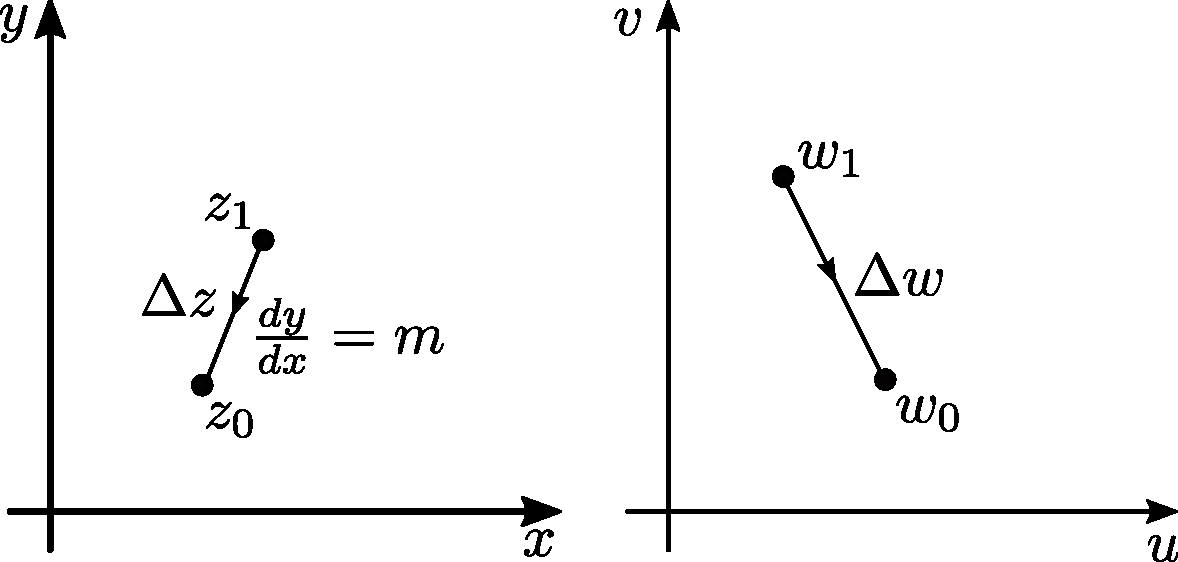
\includegraphics[width=0.9\textwidth]{figs/fig-05}

		\[ \frac{\Delta w}{\Delta z} = \frac{1 - im}{1 + im} = g(m) \]
	\end{columns}
\end{frame}

\begin{frame}{Aplicación: ecuación de Laplace y ejemplo}
	$u(x, y)$ satisface la ecuación de Laplace si:
	\[\boxed{ \frac{\partial^2 u}{\partial x^2} + \frac{\partial^2 u}{\partial y^2} = 0 } \] \pause
	\vspace{1em}

	\begin{columns}[t]
		\cx
		Si $u + i v$ es \textbf{analítica}:
		\begin{align*}
			u_x = v_y \;  & \therefore \; u_{xx} = v_{yx}  \\
			u_y = -v_x \; & \therefore \; u_{yy} = -v_{xy} \\
		\end{align*} \vspace{-3em}
		\begin{align*}
			\frac{\partial^2 u}{\partial x^2} + \frac{\partial^2 u}{\partial y^2} & = 0 \\
			\frac{\partial^2 v}{\partial x^2} + \frac{\partial^2 v}{\partial y^2} & = 0
		\end{align*} \pause

		\cx
		\begin{exampleblock}{Ejemplo:}
			\[ f(z) = z^2 \longrightarrow
				\begin{cases}
					u = x^2 - y^2 \\
					v = 2 x y
				\end{cases}
			\]

			\[
				\therefore \left. { \begin{array}{ll}
					u_{xx} + u_{yy} & = 0 \\
					v_{xx} + v_{yy} & = 0
				\end{array} }
				\right\}
			\]
		\end{exampleblock}
	\end{columns}
\end{frame}

\begin{frame}[standout]
	Pausa para resolver problemas: 9 -- 13.
\end{frame}


\section{Integración de funciones complejas}
\begin{frame}{Integración de funciones complejas}
	\begin{columns}[t]

		\cw{0.35}

		\textbf{Revisión:}
		\[ \int_{x_0}^{x_1} f(x) \, dx = \lim_{\substack{\max \\ \Delta x \rightarrow 0}} \sum_{k=1}^n f(c_k^*) \Delta x_k \]


		\[ = F(x_1) - F(x_0), \; F' = f \]


		\begin{center}
			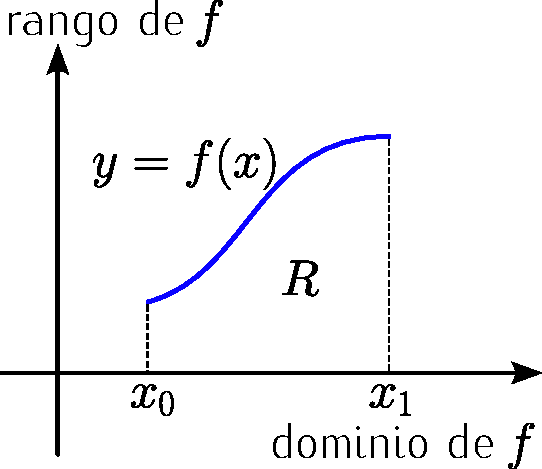
\includegraphics[width=0.85\textwidth]{figs/fig-06.pdf}
		\end{center}
		\pause

		\cw{0.35}
		\phantom{alineación de ecuaciones}

		\[ \int_{z_0}^{z_1} f(z) \, dz \overset{{\color{red}{?}}}{=} \lim_{\substack{\max \\ \Delta z \rightarrow 0}} \sum_{k=1}^n f(c_k^*) \overset{{\color{red}{?}}}{\Delta z_k} \]

		\[ C: \begin{cases}
				x = x(t) \\
				y = y(y) \\
			\end{cases} =
			\begin{cases}
				\vec{R} = x(t) \hat{i} + y(t) \hat{j} \\
				z = x(t) + i y(t)                     \\
			\end{cases} \]

		$\qquad t_0 \leq t \leq t_1$

		\begin{multline*} \int_{C: z_0}^{z_1} f(z) \, dz = \lim_{\substack{\max \\ \Delta z \rightarrow 0}} \sum_{k=1}^n f(c_k(t_k)) \frac{\Delta z_k}{\Delta t_k} \Delta t_k \\
			\therefore \int_{C: z_0}^{z_1} f(z) \, dz = \int_{t_0}^{t_1} f(z(t)) z'(t) \, dt
		\end{multline*}

		\cw{0.25}
		\vspace{2em}
		\begin{center}
			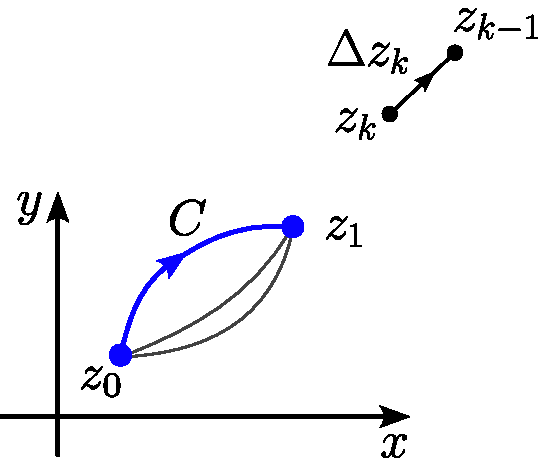
\includegraphics[width=0.85\textwidth]{figs/fig-07.pdf}
		\end{center}
	\end{columns}
\end{frame}

\begin{frame}
	\begin{columns}[t]
		\cw{0.45}
		En términos de $u$ y $v$: $f(z) = u + i v$, $\Delta z = \Delta x + i \Delta y$:
		\begin{multline*}
			\int_{\substack{C \\z_0}}^{z_1} f(z) \, dz = \int_{\substack{C \\ (x_0, y_0)}}^{(x_1, y_1)} (u + i v)(dx + i dy) = \\
			\int_{\substack{C \\ (x_0, y_0)}}^{(x_1, y_1)} (u \, dx - v \, dy) + i \int_{\substack{C \\ (x_0, y_0)}}^{(x_1, y_1)} (v \, dx + u \, dy) \\
			C: \begin{cases}
				x = x(t) \\
				y = y(t)
			\end{cases}
		\end{multline*}

		Si $u + i v$ es \alert{analítica}: $u_x = v_y, \; u_y = -v_x$.

		\[ \therefore \begin{rcases*}
				u \, dx - v \, dy \\
				v \, dx + u \, dy
			\end{rcases*} \text{ es diferencial exacta.} \]

		\cw{0.45}

		$\therefore$ Si $f = u + i v$ en analítica:
		\[ \int_{z_0}^{z_1} f(z) \, dz \]
		es \textbf{independiente} de $C$, y
		\[ \boxed{ \oint_C f(z) \, dz = 0, \quad \forall C} \]

		$f$ analítica $\rightarrow$
		\[ \int_{z_0}^{z_1} f(z) \, dz = F(z_1) - F(z_0), \quad F' = f \]

		\begin{alertblock}{Nota:}
			\[ \oint_C f(z) \, dz \]
			\textbf{no necesariamente es 0} si $f$ no es analítica.
		\end{alertblock}
	\end{columns}
\end{frame}

\begin{frame}{Ejemplo}
	\begin{columns}[t]
		\cw{0.3}
		Calcular: \[ \oint_C \frac{dz}{z} \]
		donde
		\begin{center}
			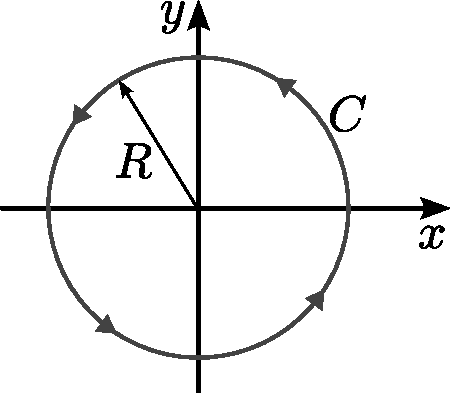
\includegraphics[width=0.75\textwidth]{figs/fig-08.pdf}
		\end{center}
		El integrando es analítico en $\mathbb{C}$ excepto en $z = 0$.

		\cw{0.3}
		Método \#1:
		\begin{multline*}
			\oint_C \frac{dz}{z} = \oint_C \frac{dx + i dy}{x + i y} \\
			= \oint_C \frac{(x-iy)(dx + i dy)}{x^2 + y^2} = \\
			\oint_C\frac{x \, dx + y \, dy}{x^2 + y^2} + i \oint_C \frac{-y \, dx + x \, dy}{x^2 + y^2}
		\end{multline*}
		En $C$: $x = R \cos \theta, \, y = R \sen \theta$, $dx = -R \sen \theta \, d\theta$, \\ $dy = R \cos \theta \, d\theta$, $x^2 + y^2 = R^2, \, 0 \leq \theta \leq 2 \pi$.
		\begin{multline*}
			\therefore \oint_C \frac{dz}{z} = 0 \\
			+ i \int_0^{2 \pi} \frac{R^2(\sen^2 \theta + \cos^2 \theta) \, d\theta}{R^2} \\
			= \boxed{2 \pi i}
		\end{multline*}
		\pause

		\cw{0.3}
		Método \#2:
		$C: z = R e^{i \theta}, \; 0 \leq \theta \leq 2 \pi$.
		\begin{multline*}
			\frac{dz}{d\theta} = i R e^{i \theta} \\
			\oint_C \frac{dz}{z} = \int_0^{2 \pi} \frac{1}{z(\theta)} \frac{dz}{d\theta} d\theta \\
			= \int_0^{2 \pi} \frac{i R e^{i \theta}}{R e^{i \theta}} d\theta \\
			= \boxed{2 \pi i}
		\end{multline*}
	\end{columns}
\end{frame}

\begin{frame}
	\begin{columns}[t]
		\cx
		Geometría elástica (topología):
		\begin{center}
			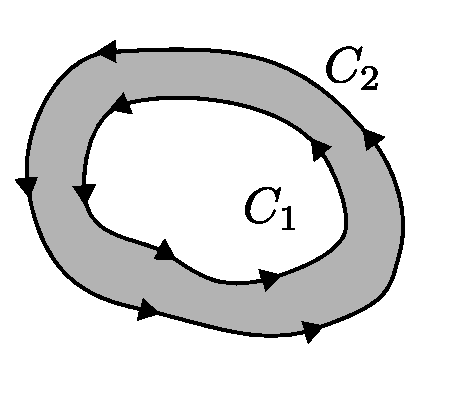
\includegraphics[scale=0.45]{figs/fig-09.pdf}
		\end{center}

		Si $f$ es analítica en $C_1$ y $C_2$, y en la región entre ellas, entonces:
		\[ \oint_{C_1} f(z) \, dz = \oint_{C_2} f(z) \, dz \]
		\begin{center}
			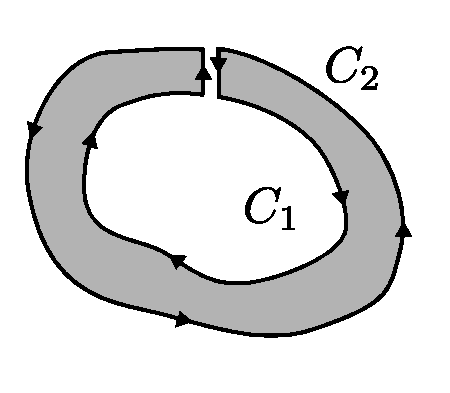
\includegraphics[scale=0.45]{figs/fig-09b.pdf}
		\end{center}

		\cx
		\[\oint_{\cancel{C}} f(z) \, dz = \oint_{C_2} f(z) \, dz - \oint_{C_1} f(z) \, dz = 0 \]
		\pause

		\textbf{Ejemplo:} calcular
		\[ \oint_C \frac{dz}{z} \]
		donde
		\begin{center}
			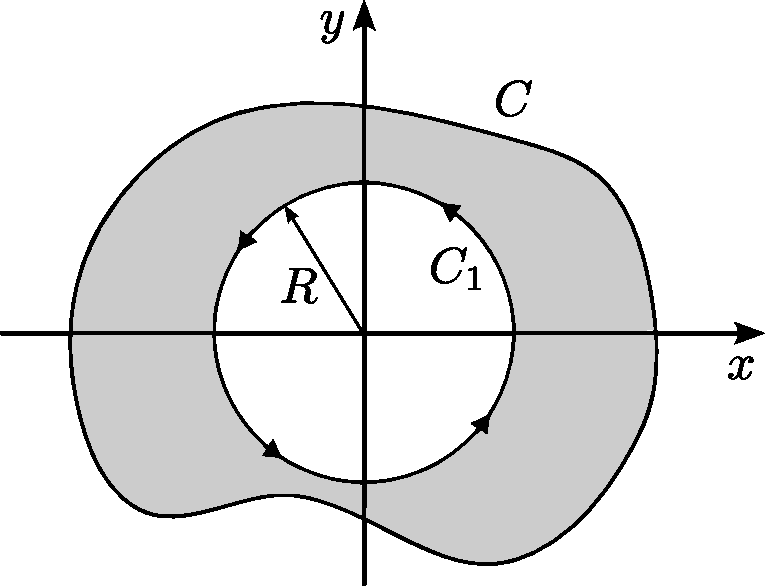
\includegraphics[scale=0.40]{figs/fig-10.pdf}
		\end{center}

		\[ \oint_C \frac{dz}{z} = \oint_{C_1} \frac{dz}{z} = 2 \pi i \]

	\end{columns}
\end{frame}


\begin{frame}[standout]
	Pausa para resolver problemas: 14 -- 17.
\end{frame}

\section{Secuencias y series}

\begin{frame}[t]
	\frametitle{Secuencias y series}
	\begin{columns}[t]
		\cw{0.3}
		\[ e^z = ?, \qquad \sen z = ? \]
		\begin{align*}
			e^x & = \sum_{n = 0}^{\infty} \frac{x^n}{n!}                      \\
			e^z & = \sum_{n = 0}^{\infty} \frac{z^n}{n!} = \textcolor{red}{?} \\
		\end{align*}
		\begin{definition}
			\vspace{-0.5em}
			\[ \lim_{n \rightarrow \infty} a_n = L \text{ significa que} \]
			dado $\varepsilon > 0, (\varepsilon \in \mathbb{R})$, existe $N$, tal que \vspace{-0.5em}
			\[ n > N \rightarrow |a_n - L| < \varepsilon \]

		\end{definition}

		\cw{0.3}
		Gráficamente:
		\begin{center}
			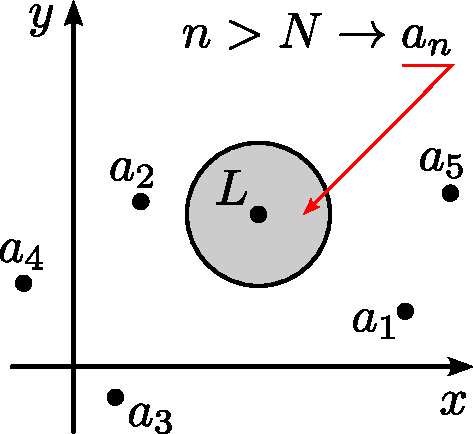
\includegraphics[scale=0.35]{figs/fig-11.pdf}
		\end{center}
		En forma similar podemos definir:
		\[ \sum_{n = 1}^{\infty} c_n = \lim_{n \rightarrow \infty} (c_1 + \cdots + c_n) \]

		Por su estructura, \textbf{son válidos} todos los teoremas usuales.

		\cw{0.3}
		En particular, si $S = \{ z: \sum a_n z^n \text{ converge } \} $, entonces pueden darse los siguientes casos:
		\begin{enumerate}[i)]
			\item $ S = \{ 0\} $.
			\item $S = \mathbb{C} $ (todos los números complejos).
			\item Existe un $R > 0$ tal que $S = \{z: |z| < R \} $, y la convergencia es absoluta e uniforme para $|z| \leq r < R$.
		\end{enumerate}
		\begin{center}
			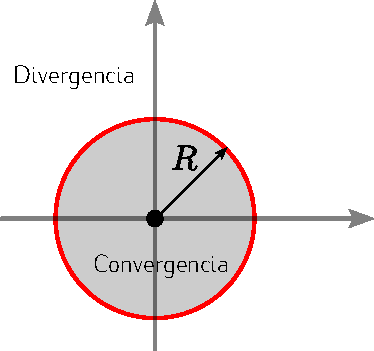
\includegraphics[scale=0.35]{figs/fig-12.pdf}
		\end{center}
	\end{columns}
\end{frame}

\begin{frame}
	\begin{columns}[t]
		\cw{0.3}
		Entonces podemos \textbf{definir}:
		\begin{align*}
			e^z    & = \sum_{n = 0}^{\infty} \frac{z^n}{n!}                      \\
			\sen z & = \sum_{n = 0}^{\infty} \frac{(-1)^n z^{2 n + 1}}{(2n +1)!} \\
			\sen x & = \sum_{n = 0}^{\infty} \frac{(-1)^n x^{2 n + 1}}{(2n +1)!} \\
		\end{align*}
		Se puede entonces probar que:
		\begin{align*}
			e^{iz}                 & = \cos z + i \sen z               \\
			                       & \text{o}                          \\
			e^{ix}                 & = \cos x + i \sen x               \\
			\therefore (r, \theta) & = r \cos \theta + i r \sen \theta \\
			                       & = r e^{i \theta}
		\end{align*}

		\cw{0.3}
		Tres observaciones:
		\begin{enumerate}
			\item $z = r e^{i \theta} = r e^{i(\theta + 2 \pi k)} $
			      \begin{align*}
				      \therefore \log z & = \log r + \log e^{i(\theta + 2 \pi k)} \\
				                        & = \ln r + i (\theta + 2 \pi k)
			      \end{align*}
			      $\therefore \log z$ es multivaluada, el \textbf{valor principal} es $-\pi < \theta \leq \pi$.
			\item
			      \begin{multline*}
				      \cosh i x = \frac{e^{ix} + e^{-ix}}{2} = \\
				      \frac{(\cos x + i \sen x)}{2} + \\
				      \frac{\cos(-x) + i \sen(-x)}{2} = \cos x
			      \end{multline*}
		\end{enumerate}

		\cw{0.3}
		\begin{enumerate}
			\setcounter{enumi}{2}
			\item $e^z = e^{x + i y} = e^x e^{iy} =$
			      \begin{multline*}
				      e^x (\cos y + i \sen y) = \\
				      e^x \cos y + i e^x \sen y \\
				      u(x, y) + i v(x, y)
			      \end{multline*}
		\end{enumerate}
		$u$ y $v$ representan un \textbf{mapeo conforme} real:
		\begin{center}
			\begin{overprint}
				\onslide<1>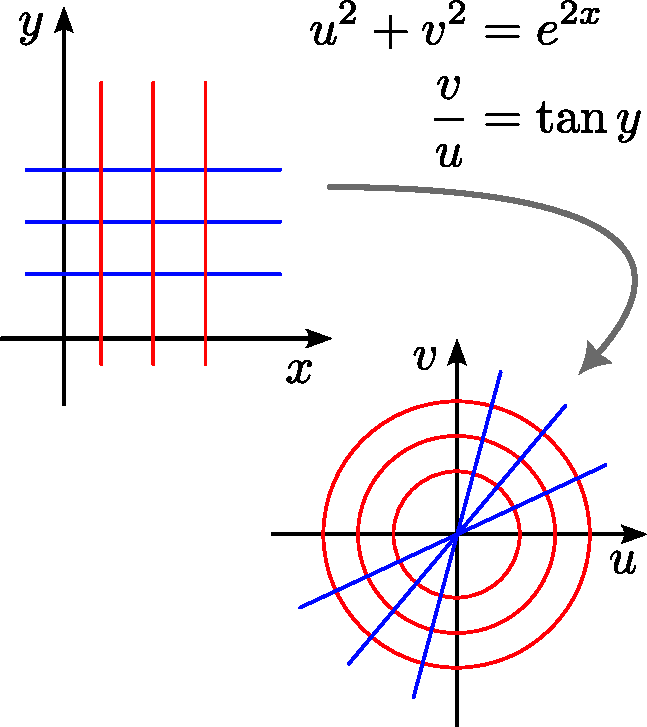
\includegraphics[width=0.95\textwidth]{figs/fig-13.pdf}
				\onslide<2>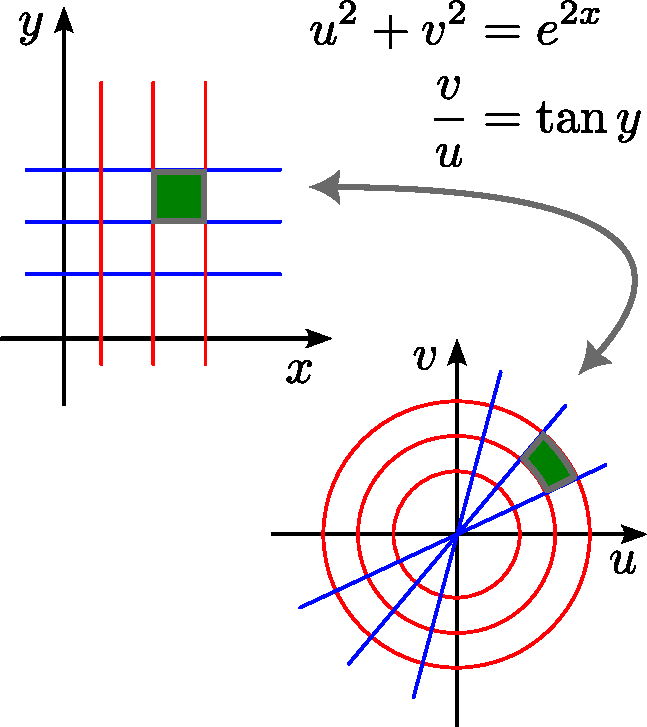
\includegraphics[width=0.95\textwidth]{figs/fig-13b.pdf}
			\end{overprint}
		\end{center}
	\end{columns}
\end{frame}

\begin{frame}{Aplicación a series ``reales''}
	\begin{columns}[c]
		\cw{0.3}
		\begin{align*}
			\frac{1}{1 - u} & = 1 + u + u^2 + \cdots      \\
			                & = \sum_{n = 0}^{\infty} u^2
		\end{align*}
		converge para $|u| < 1$.
		\begin{align*}
			\therefore \frac{1}{1 + x^2} & = 1 - x^2 + x^4 - x^6 + \cdots    \\
			                             & = \sum_{n}^{\infty} (-1)^n x^{2n}
		\end{align*}
		converge para $|x| < 1$.
		\cw{0.3}
		¿Qué pasa en $x = \pm 1$?
		\begin{align*}
			\sum_{n = 0}^{\infty} (-1)^n z^{2n} & = \frac{1}{1 + z^2}, \; ({\color{red}|z| < 1}) \\
			\frac{1}{1 + z^2}                   & = \frac{1}{(z + i)(z -i)}
		\end{align*}
		$\therefore z = \pm i \leftarrow $ \alert{¡problema!}
		\cw{0.3}
		Gráficamente:
		\begin{center}
			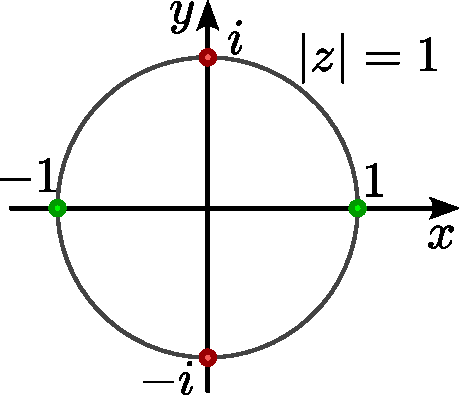
\includegraphics[scale=0.40]{figs/fig-14.pdf}
		\end{center}
		Los puntos problemáticos están \textbf{sobre} $|z| = 1$, pero no en $z = 1$ o en $z = -1$.
	\end{columns}
\end{frame}


\begin{frame}[standout]
	Pausa para resolver problemas: 18 -- 19.
\end{frame}



\section*{Bibliografía}
\begin{frame}{Lecturas recomendadas}
	\begin{itemize}
		\item \fullcite{kreyszig2011}. Capítulo 13 - 16.
		\item \fullcite{spiegel2011}. Capítulos 1, 2, 6, 14.
	\end{itemize}
	% \nocite{kreyszig2011}
	% \nocite{spiegel2011}
	% \nocite{vesely2012}
	% \nocite{thornton2015}
	% \printbibliography
\end{frame}
\end{document}

